\subsection{Data Visualisation/Representation}
\label{sec:DV}
\begin{tcolorbox}[title=Analysis in the Modern Age]
Discovery is no longer limited by the collection and processing of data, but rather management, analysis, and visualisation. \\[-0.6cm]
\begin{flushright}
-- @DamienMingle
\end{flushright}
\end{tcolorbox}
\noindent What can be done with the data, once it has been collected? Two suggestions come to mind: 
\begin{itemize}[noitemsep,topsep=2pt]
\item \textbf{analysis} is the process by which we extract actionable insights from the data (this process is discussed in later subsections), while
\item \textbf{visualisation} is the process of presenting data, calculations, and analysis outputs in a visual format. Visualisation of data \textit{prior} to analysis can help simplify the analytical process. Visualisation \textit{following} analysis allows for the analysis results to be presented to various stakeholders.  
\end{itemize}
\vspace{3pt}
In this section, we focus on important visualisation concepts and methods; we shall provide examples of data displays to illustrate the various possibilities that might be produced by the data presentation component of a data analysis system.   
\subsubsection{Pre-Analysis Use}
\begin{tcolorbox}[title=The Ying.. ]
A picture is worth a thousand words.\\[-0.6cm]
\begin{flushright}
-- ancient saying
\end{flushright}
\end{tcolorbox}\noindent Even before the analytical stage is reached, data visualisation can be used to set the stage for analysis by:
\begin{itemize}[noitemsep,topsep=2pt]
\item detecting invalid entries and outliers,
\item shaping the data transformations (binning, standardisation, Box-Cox transformations, dimension reduction, etc.),
\item getting a sense for the data (data analysis as an art form, exploratory analysis), and 
\item identifying hidden data structures (clustering, associations, patterns which may inform the next stage of analysis, etc.)
\end{itemize}
\subsubsection{Presenting Results}
\begin{tcolorbox}[title=... and the Yang]
A thousand and one words are worth more than a picture.\\[-0.6cm]
\begin{flushright}
-- John McCarthy (attributed)
\end{flushright}
\end{tcolorbox}\noindent
The crucial element of data presentations is that they need to help convey the insight or the message. To that effect, they should be clear, engaging, and (more importantly) readable. Our ability to think of questions (and to answer them) is in some sense limited by what we can visualise. There is always a danger that if certain types of visualisation techniques dominate the evidence presentations, the kinds of questions that are particularly well-suited to providing data for these techniques will come to dominate the landscape, which will then affect data collection techniques, data availability, future interest, and so forth.
\paragraph{Generating Ideas and Insights} In \textit{Beautiful Evidence} \cite{DV_T2}, Edward Tufte explains that evidence is presented to assist our thinking processes. He further suggests that there is a symmetry to visual displays of evidence -- the consumers should be seeking exactly what the producers should be providing, namely:
\begin{itemize}[noitemsep, topsep=2pt]
\item meaningful comparisons
\item causal networks and underlying structure
\item multivariate links
\item integrated and relevant data
\item a primary focus on content
\end{itemize}
\vspace{3pt}
The choice of visualisation methods is strongly dependent on the analysis objective, that is, on the questions that need to be answered. The presentation method should not be selected randomly (or simply from a list of easily-produced templates). \newl In Figure~\ref{fig:5W},
\begin{figure}[!t]
\centering
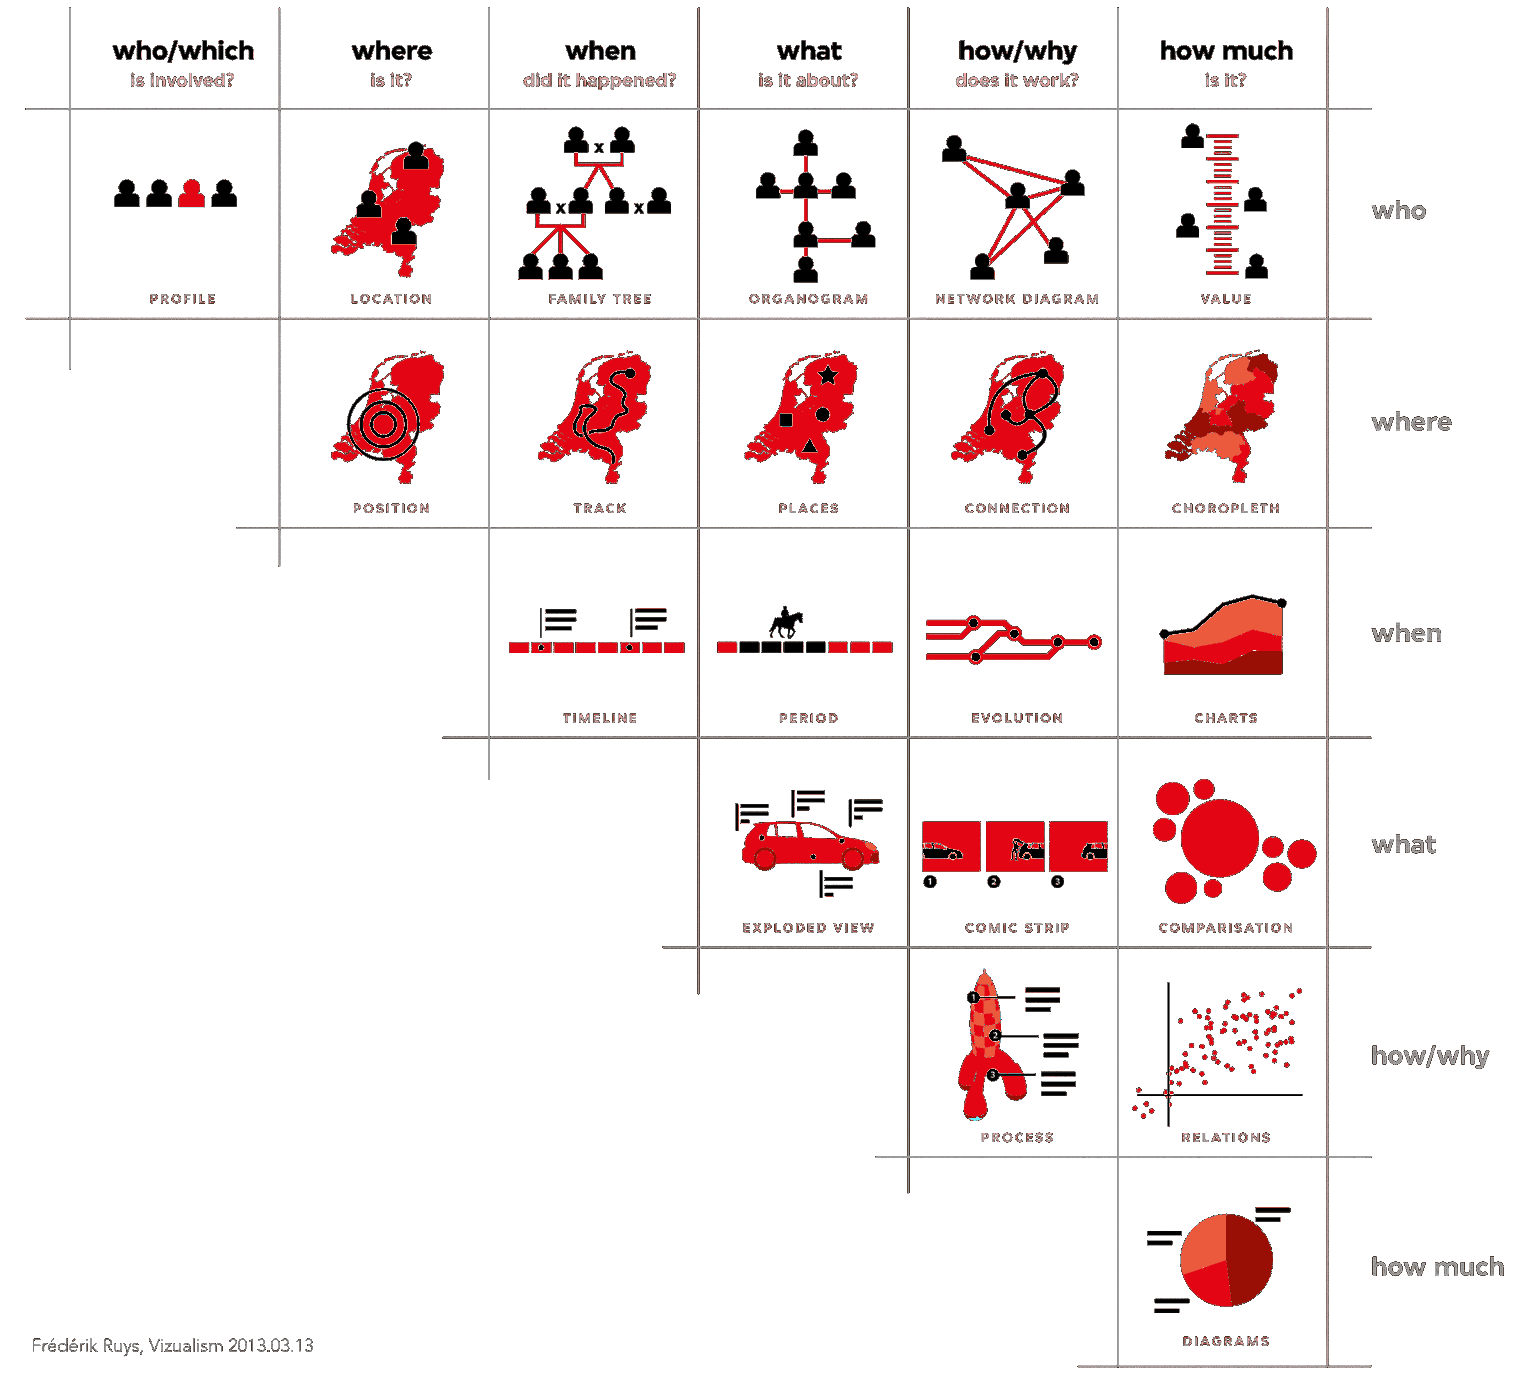
\includegraphics[width=\textwidth]{images/DV/5W_Ruys.png}
\caption[\small Data visualisation suggestions, by type of question ]{\small Data visualisation suggestions, by type of question (F.Ruys, Vizualism).} \hrule\label{fig:5W}
\end{figure}
 Fr\'ed\'erik Ruys suggests various types of visual displays that can be used, depending on the questions that are being asked: \\ \bigskip  
\begin{minipage}{\textwidth}
\begin{multicols}{2}
\begin{itemize}[noitemsep]
\item who is involved?
\item where is it taking place? 
\item when did it happen? 
\item what is it about? 
\item how/why does it work? 
\item how much? 
\end{itemize}\end{multicols}\end{minipage}\newl
A general dashboard should at least be able to produce the following types of display: 
\begin{itemize}[noitemsep,topsep=0pt]
\item \textbf{charts} -- comparison and relation (scatterplots, bubble charts, parallel coordinate charts, decision trees, cluster plots, trend plots) 
\item \textbf{choropleth maps} (heat maps, classification maps)  
\item \textbf{network diagrams} and connection maps (association rule networks, phrase nets)
\item \textbf{univariate diagrams} (word clouds, box plots, histograms) 
\end{itemize}  
\subsubsection{Multivariate Elements in Charts}
\label{appendix:datapresentation}
\begin{tcolorbox}[title=Cubism's Missing Link]
Picasso was particularly struck by Poincar\'e's advice on how to view the fourth dimension, which artists considered another spatial dimension. If you could transport yourself into it, you would see every perspective of a scene at once. But how to project these perspectives on to canvas?\\[-0.6cm]
\begin{flushright}
-- John McCarthy (attributed)
\end{flushright}
\end{tcolorbox}\noindent
At most two fields can be represented by position in the plane. How can we then represent other crucial elements on a flat computer screen? \newpage\noindent Potential solutions include: \\ \bigskip  
\begin{minipage}{\textwidth}
\begin{multicols}{2}
\begin{itemize}[noitemsep]
\item third dimension
\item marker size
\item marker colour
\item colour intensity and value 
\item marker texture
\item line orientation
\item marker shape
\item motion/movie
\end{itemize}\end{multicols}\end{minipage}\newl These elements do not always mix well -- efficient design is as much art as it is science. 
% In \textit{Semiology of Graphics}, Jacques Bertin suggests that not all of those retinal variables are equally effective in their ability to convey information. Some of their strengths are shown in Figure~\ref{fig:retinal}. \begin{figure}[t]
%\centering
%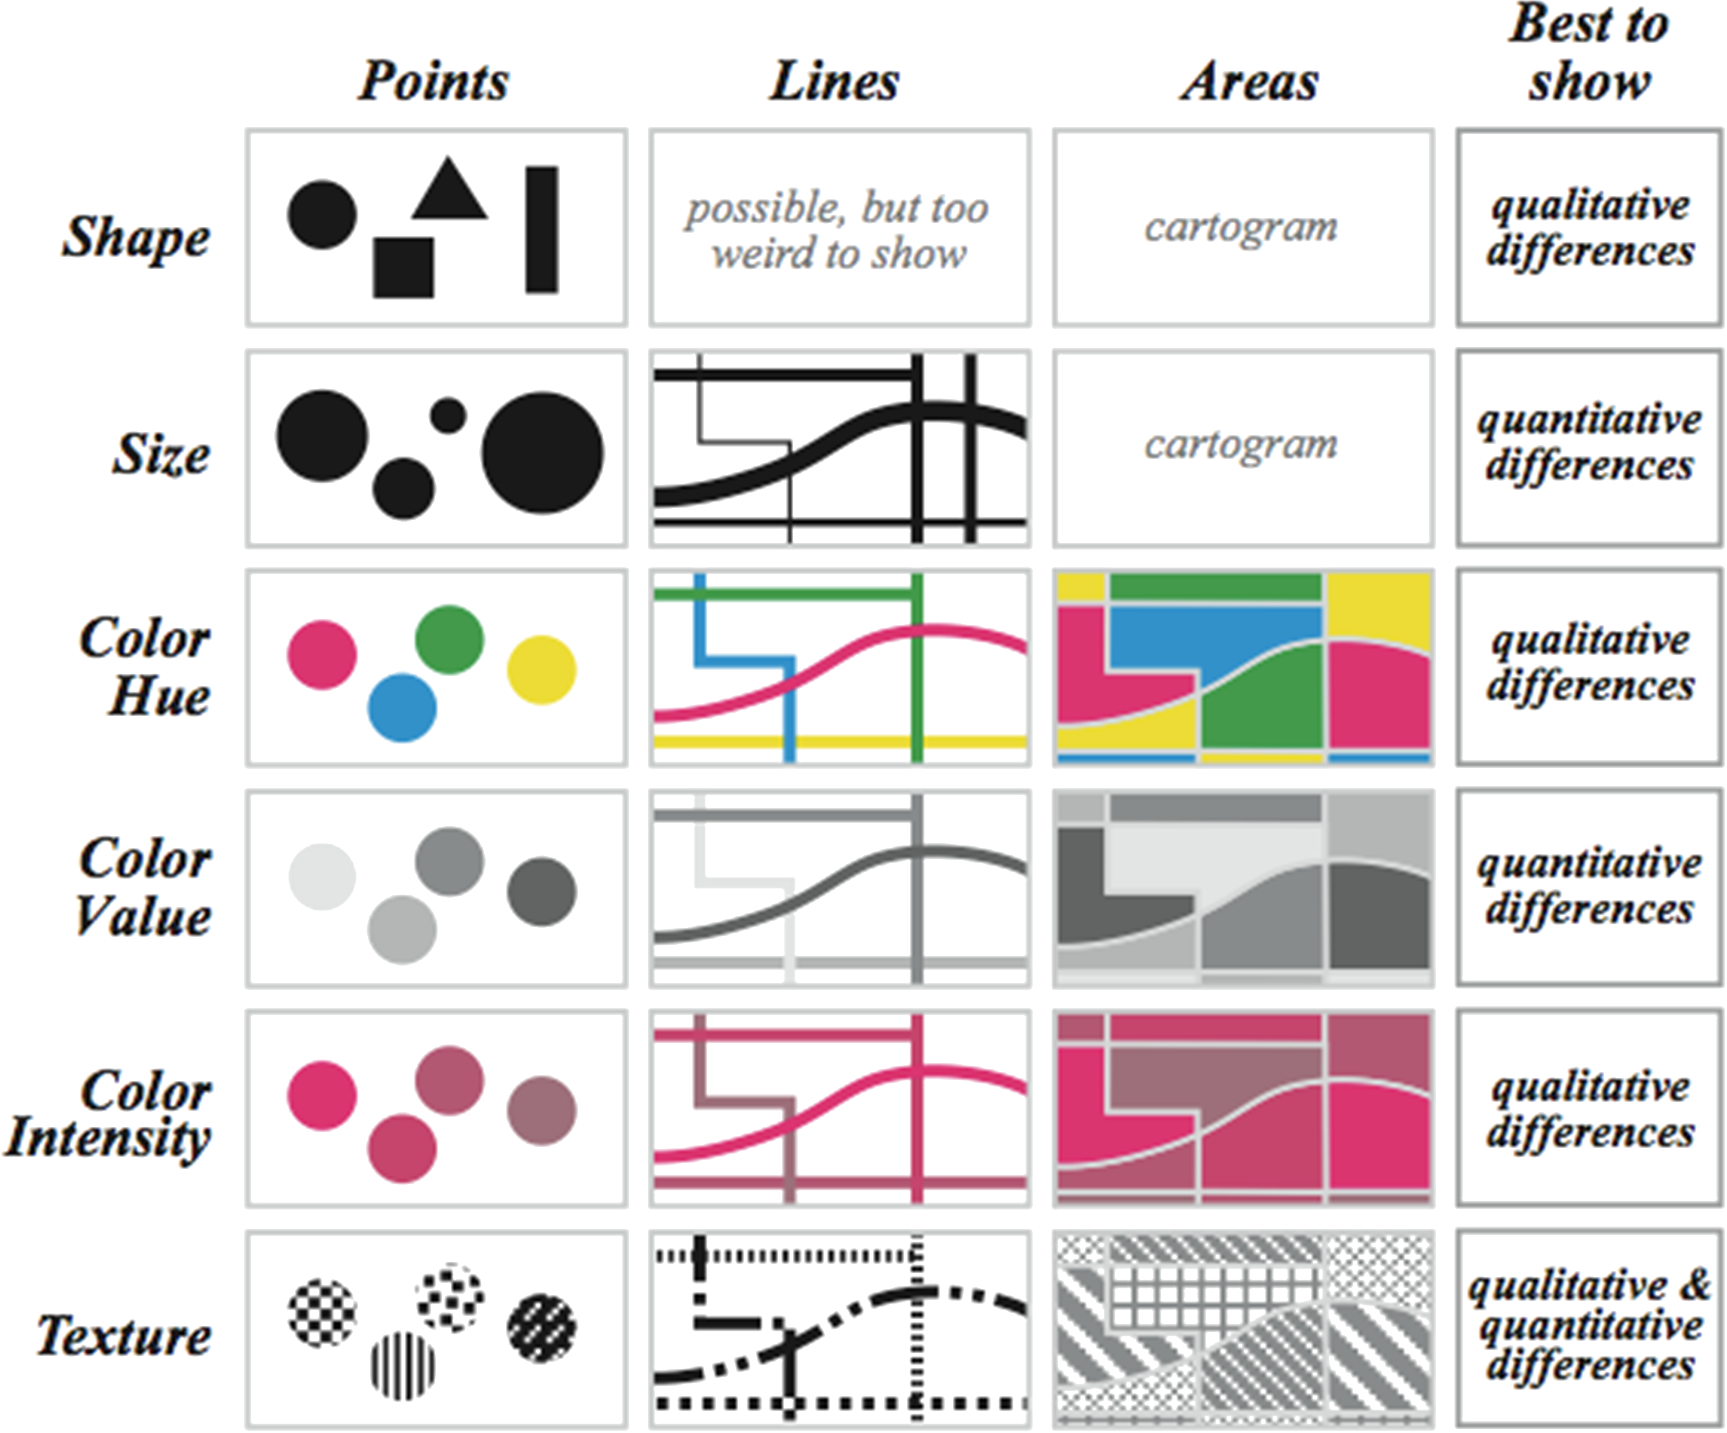
\includegraphics[width=0.8\textwidth]{images/DV/viz_retinal.png}
%\caption[\small  visualisation elements and comparisons ]{\small visualisation elements and comparisons (J.Krygier, D.Wood).} \hrule\label{fig:retinal}
%\end{figure}
%\afterpage{\FloatBarrier}
\paragraph{Examples} In what follows, we provide examples for each of these chart types, along with a concise description of key components and a list of questions that they could help answer for four of them. Some additional diagrams showcasing the four presentation types discussed previously are highlighted in Figures~\ref{fig:ex_dt_kyp} to \ref{fig:ex_ts_cv}.
\begin{figure}[H]
\centering
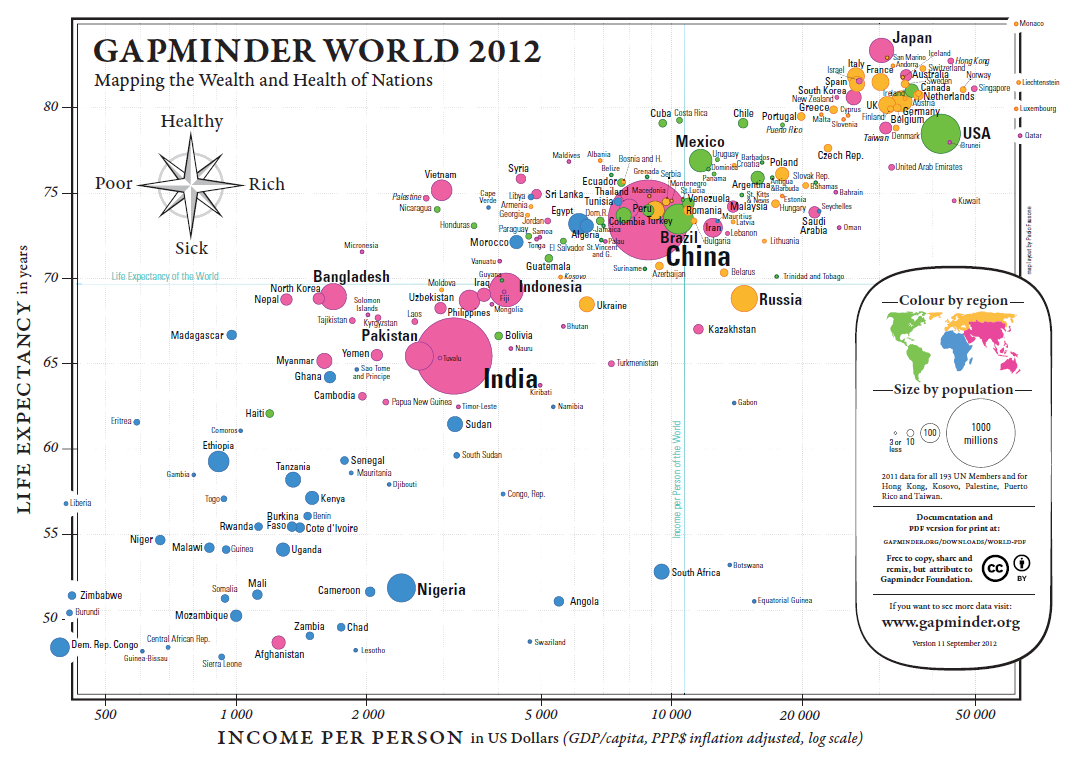
\includegraphics[width=0.92\textwidth]{images/DV/GapminderMap-2.png}
\caption[\small Bubble Chart: Gapminder's Health and Wealth of Nations ]{\small Gapminder's Health and Wealth of Nations (H.Rosling).} \hrule\label{fig:ex_bc_gap}
\end{figure}
\afterpage{\FloatBarrier}
\subparagraph{Bubble Chart:} Health and Wealth of Nations  (Figure~\ref{fig:ex_bc_gap})
\begin{itemize}[noitemsep]
\item \textbf{Data:} 2011 life expectancy in years, inflation adjusted GDP/capita in USD, population for 193 UN members and 5 other countries. 
\item \textbf{Some Questions and Comparisons:} Can we predict the life expectancy of a nation given its GDP/capita? (\textit{The trend is roughly linear: $\mbox{Expectancy}\approx 6.8 \times \ln \mbox{GDP/capita} + 10.6$}) \par Are there outlier countries? (\textit{South Africa, Botswana, and Vietnam, at a glance})\par Are countries with a smaller population healthier? (\textit{Bubble size seems uncorrelated with the axes' variates}) \par Is continental membership an indicator of health and wealth levels? (\textit{There is a clear divide between Western Nations (and Japan), most of Asia, and Africa}) \par How do countries  compare against world values for life expectancy and GDP per capita? (\textit{The vast majority of countries fall in three of the quadrants -- there are very few wealthy countries with low life expectancy. China sits near the world values, which is expected for life expectancy, but more surprising when it comes to GDP/capita -- compare with India})   
\item \textbf{Multivariate Elements:} Scatterplot positions for health and wealth, bubble size for population, colour for continental membership, labels to identify the nations. 
\item \textbf{Comments:} Are life expectancy and GDP/capita appropriate proxies for health and wealth? \par A fifth element could also be added to a screen display: the passage of time. 
\item \textbf{Reference:} Image and documentation available at the Gapminder Foundation \\ https://www.gapminder.org/downloads/world-pdf/
\end{itemize}
\newpage
\begin{figure}[H]
\centering
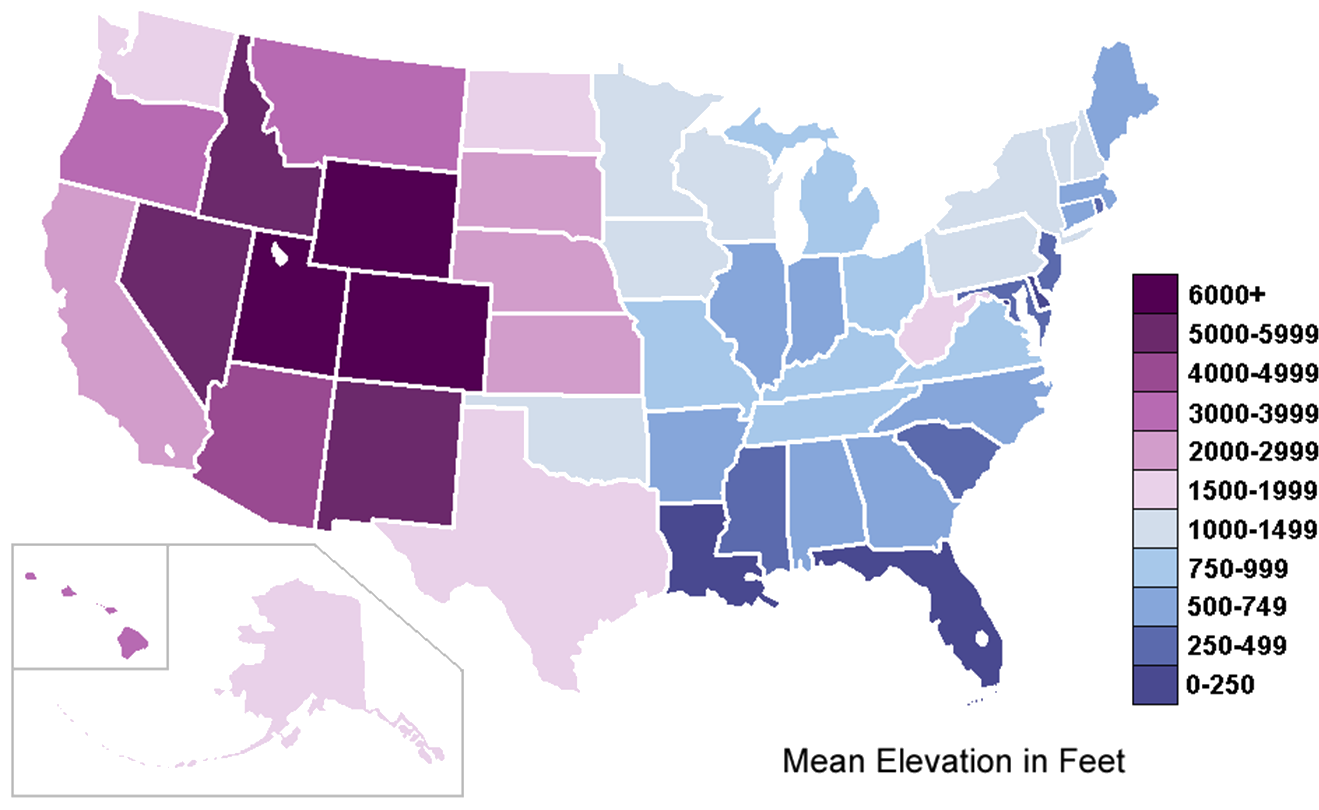
\includegraphics[width=\textwidth]{images/DV/choropleth.png}
\caption[\small Choropleth Map: mean elevation by U.S. state ]{\small Mean elevation by U.S. state, in feet (source unknown).} \hrule\label{fig:ex_ch_mef}
\end{figure}
\afterpage{\FloatBarrier}
\subparagraph{Choropleth Map:} Mean Elevation by U.S. State, in feet  (Figure~\ref{fig:ex_ch_mef})
\begin{itemize}[noitemsep]
\item \textbf{Data:} 50 observations, ranging from sea level (0-250) to (6000+)
\item \textbf{Some Questions and Comparisons:} Can the mean elevation of the U.S. states tell us something about the global topography of the U.S.? (\textit{West has higher mean elevation related to the presence of the Rockies; Eastern coastal states are more likely to suffer from rising water levels, for instance})\par Are there any states that do not ``belong'' in their local neighbourhood, elevation-wise? (\textit{West Virginia and Oklahoma seem to have the ``wrong'' shade -- is that an artifact of the colour gradient and scale in use?})  \item \textbf{Multivariate Elements:} Geographical distribution and purple-blue colour gradient (as the marker for mean elevation)
\item \textbf{Comments:} Is the `mean' the right measurement to use for this map? (\textit{it depends on the author's purpose.})\par Would there be ways to include other variables in this chart? (\textit{population density with texture, for instance})
\item \textbf{Reference:} Author unknown.
\end{itemize}
\newpage \begin{figure}[H]
\centering
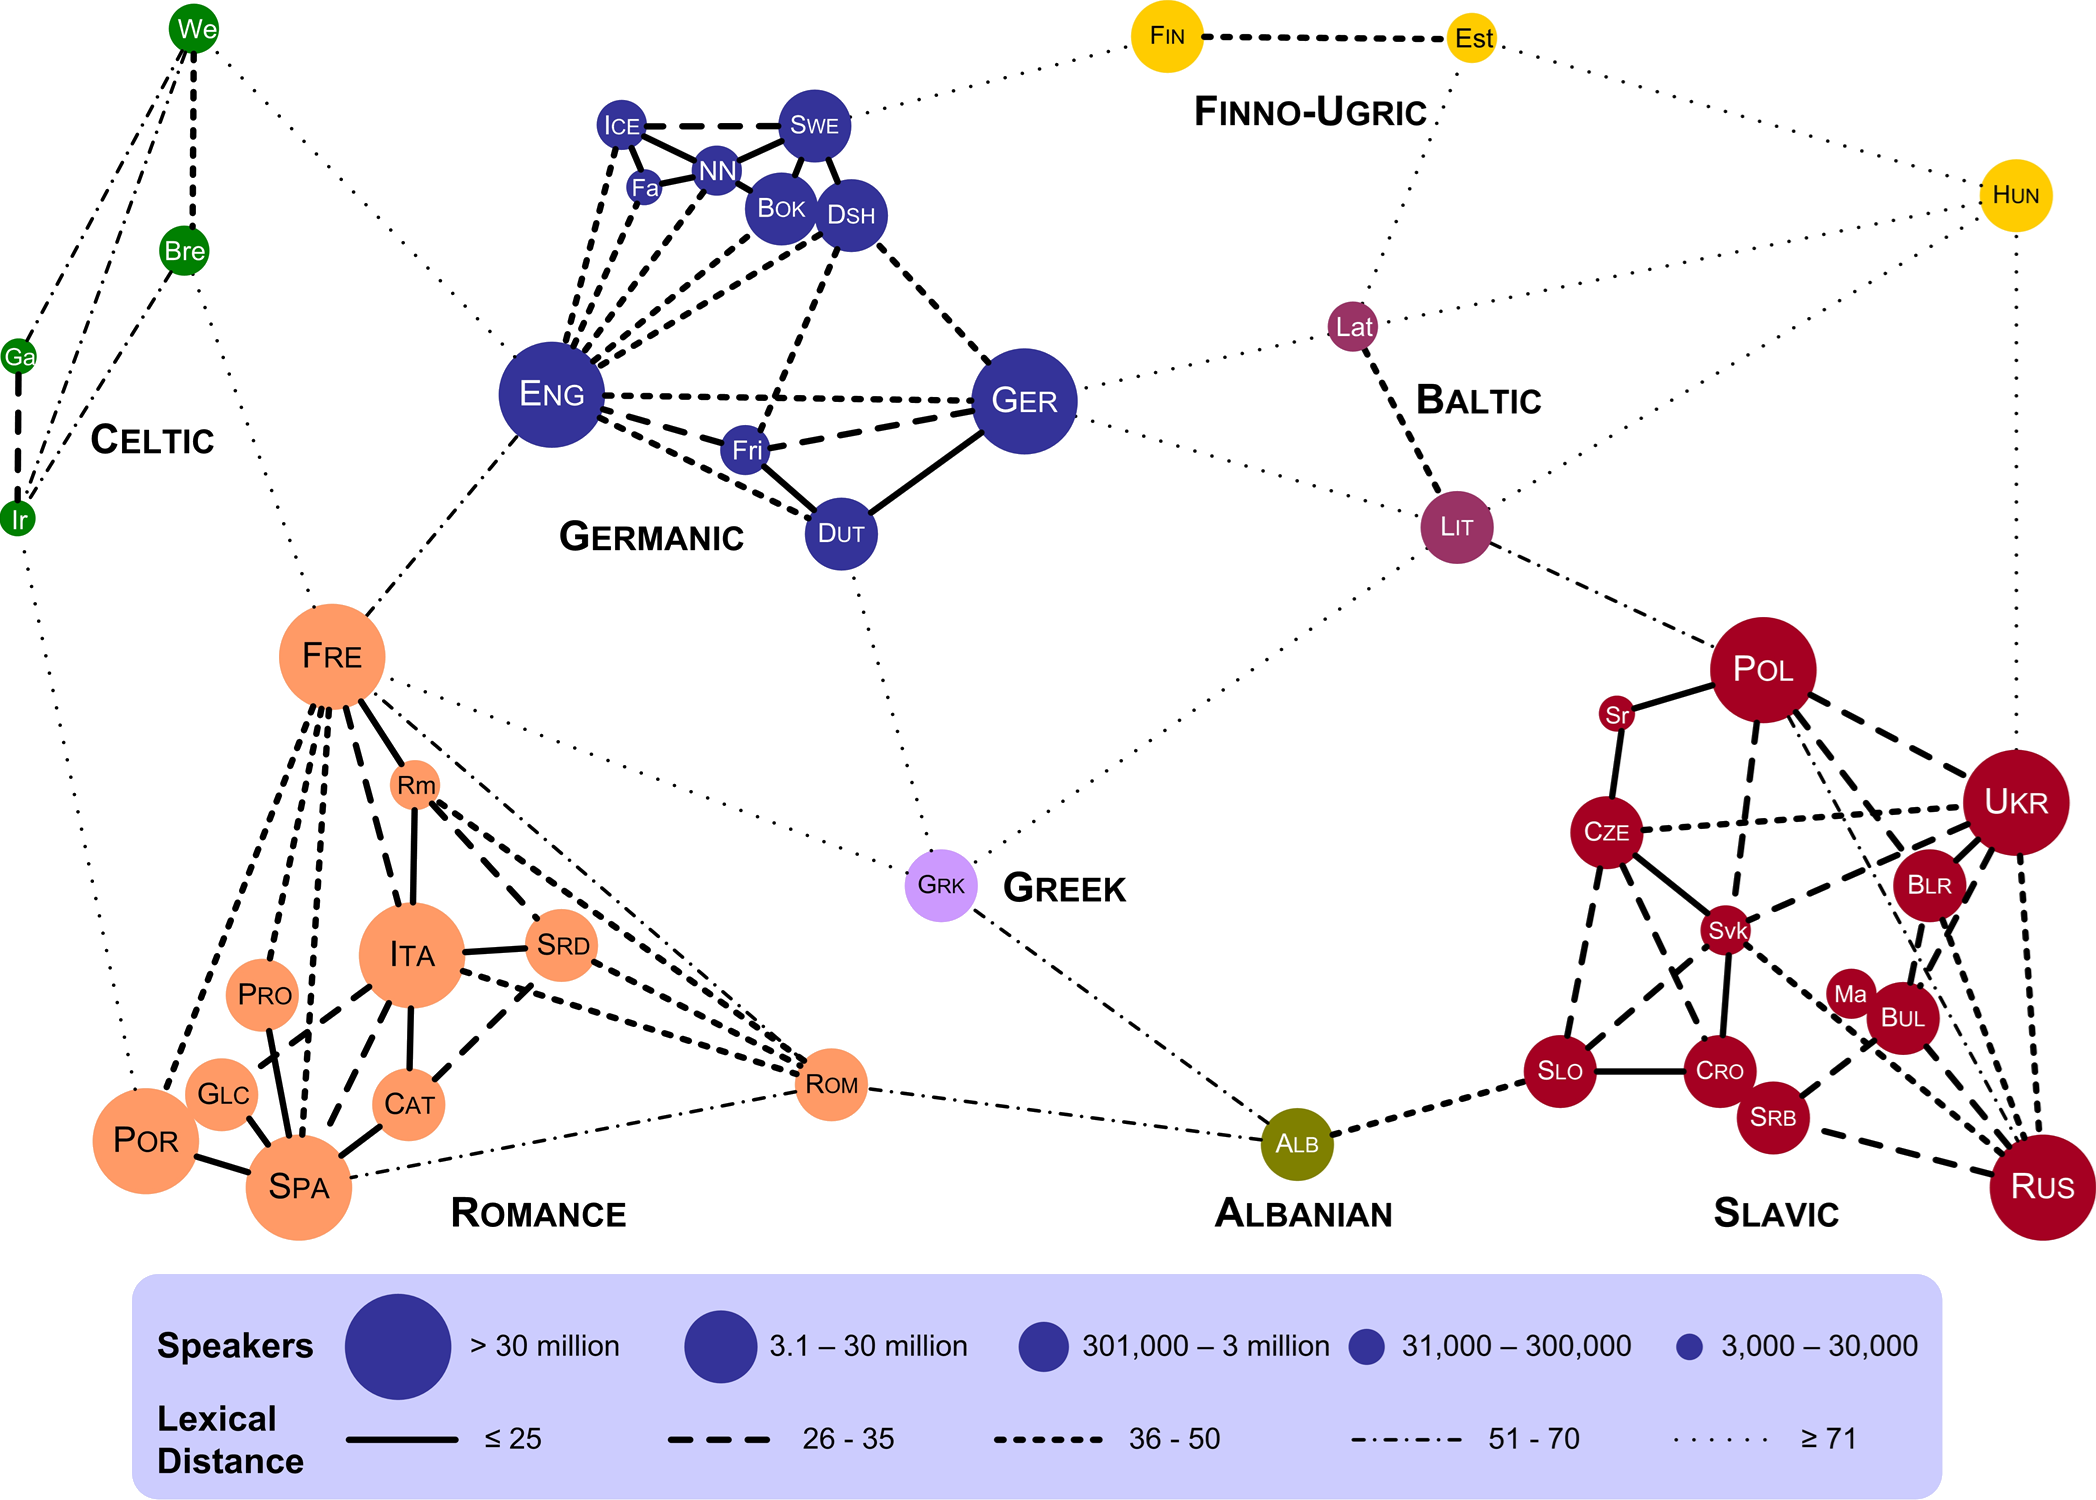
\includegraphics[width=0.95\textwidth]{images/DV/lexical.png}
\caption[\small Network Clustering: lexical distance of European languages ]{\small Lexical distance of European languages (T.Elms).} \hrule\label{fig:ex_nd_lex}
\end{figure}
\afterpage{\FloatBarrier}
\subparagraph{Network Diagram:} Lexical Distance of European Languages (Figure~\ref{fig:ex_nd_lex})
\begin{itemize}[noitemsep]
\item \textbf{Data:} Speakers and language groups for 43 European languages, lexical distances 
\item \textbf{Some Questions and Comparisons:} Are there languages that are lexically closer to languages in other lexical groups than to languages in their own groups? (\textit{French is lexically closer to English than it is to Romanian})\par Which language has the most links to other languages? \textit{(English has 10 links)} \par Are there languages that are lexically close to multiple languages in other groups? (\textit{Greek is lexically close to French (Romance), Albanian, Dutch (Germanic), and Lithuanian (Baltic)}) \par Is there a correlation between the number of speakers and the number of languages in a language group? \textit{(Language groups with more speakers tend to have more languages)}      
\item \textbf{Multivariate Elements:} Colour and cluster for language group, line style for lexical distance, bubble size for number of speakers
\item \textbf{Comments:} How is lexical distance computed?  \par Some language pairs are not joined by links -- does this mean that their lexical distance is large enough not to be rendered? \par Are the actual geometrical distances meaningful? For instance, Estonian is closer to French in the chart than it is to Portuguese -- is it also lexically closer? 
\item \textbf{Reference:} Teresa Elms, Etymologikon \\  https://elms.wordpress.com/2008/03/04/lexical-distance-among-languages-of-europe/ 
\end{itemize}

\newpage
\begin{figure}[H]
\centering
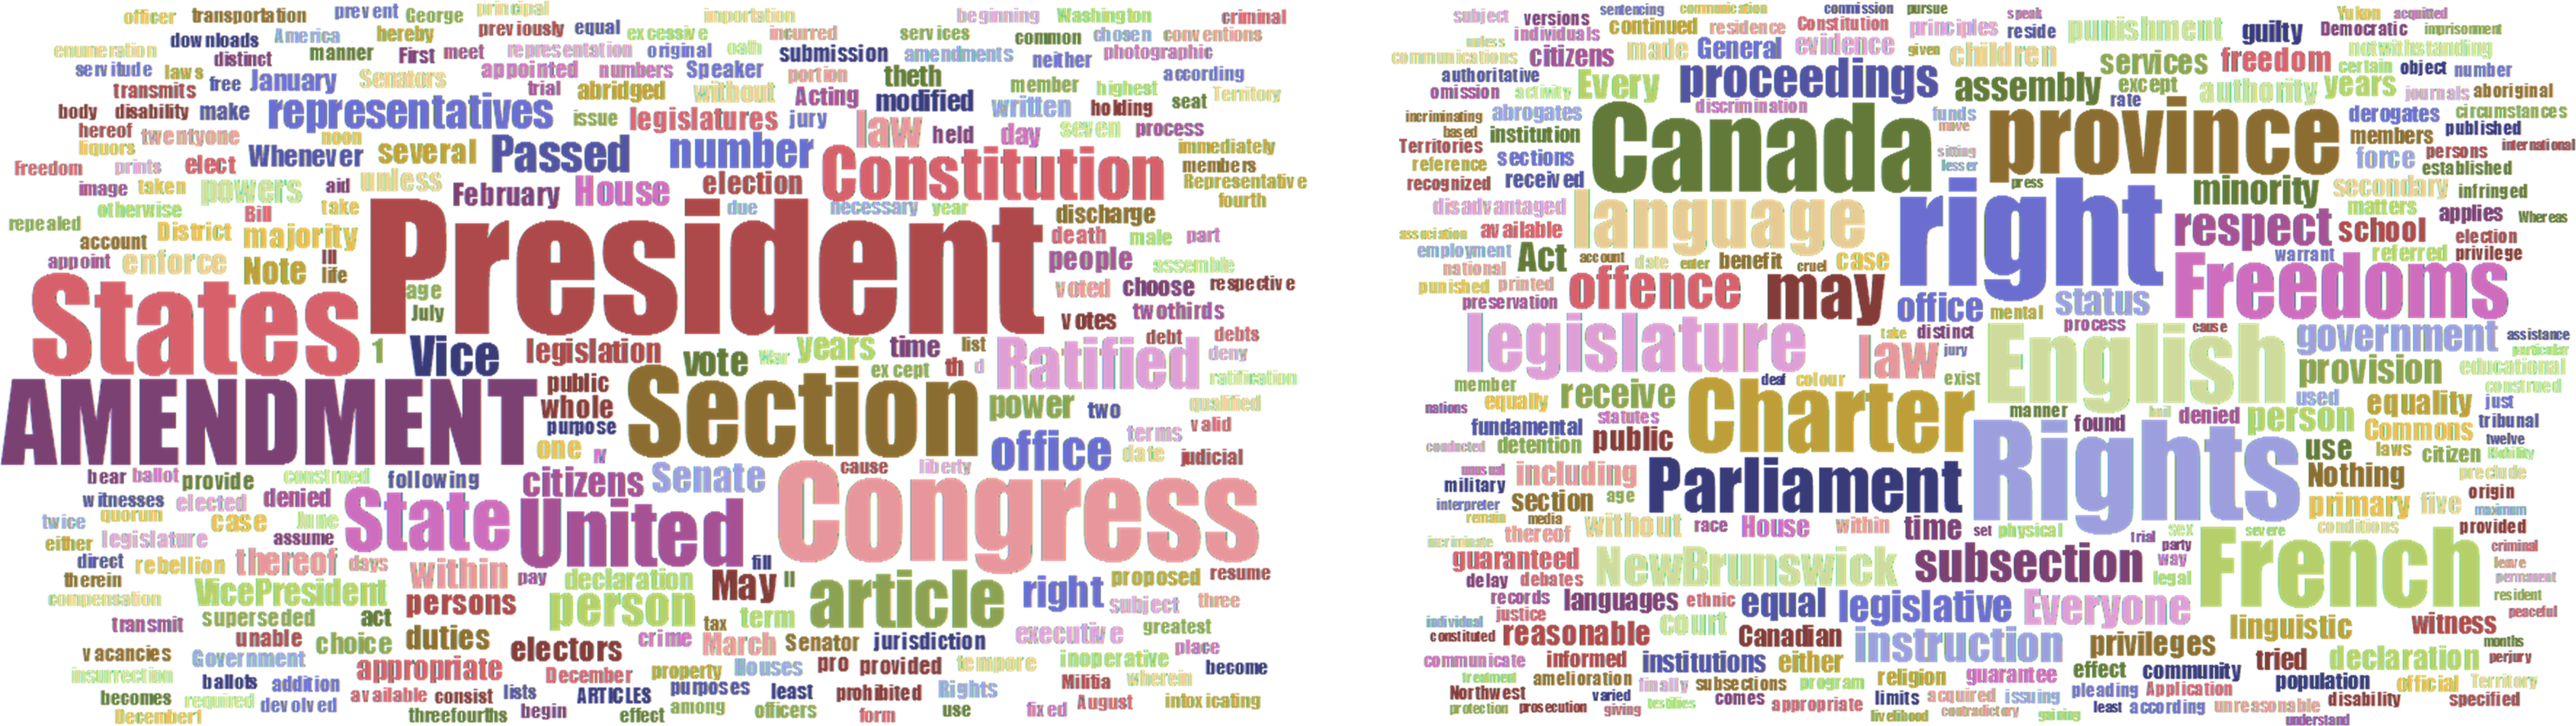
\includegraphics[width=0.9\textwidth]{images/DV/wordclouds.png}
\caption[\small Word Cloud: U.S. Constitution and Canadian Charter of Rights and Liberties ]{\small U.S. Constitution and Canadian Charter of Rights and Liberties.} \hrule\label{fig:ex_wc_UC}
\end{figure}
\afterpage{\FloatBarrier}
\subparagraph{Word Cloud:} U.S. Constitution and Canadian Charter of Rights and Liberties (Figure~\ref{fig:ex_wc_UC}).
\begin{itemize}[noitemsep]
\item \textbf{Data:} Text version of the U.S. Constitution and the Canadian Charter of Rights and Liberties 
\item \textbf{Some Questions and Comparisons:} Are these two documents of the same type? \par Do the documents have the same authors? \par Could they conceivably have been written in the same era? \par Can important differences between Canada and the U.S. be gleamed from the wordclouds? 
\item \textbf{Univariate Element:} Font size correlated with frequency count.    
\item \textbf{Comments:} Note the absence of common, content-free words (the, and, etc.). \par Colour, orientation, and word placement are not mapped to multivariate data elements in these charts, but these options are available. \par Semantic parsing and phrase nets could give us a better idea of the general ``sentiment'' underlying the documents -- what groups of words tend to occur together? \par Once the main differences have been absorbed, removing the most frequent terms from the data and producing new wordclouds on the updated texts can allow for insights regarding the setting.
\item \textbf{Reference:} Personal file.
\end{itemize}
\subsubsection{A Word About Accessibility}
\begin{tcolorbox}[title=Cubism's Missing Link]
Hear now this, O foolish people, and without understanding; which have eyes, and see not; which have ears, and hear not.\\[-0.6cm]
\begin{flushright}
-- Jeremiah 5:21 (King James Bible)
\end{flushright}
\end{tcolorbox}\noindent
While visual displays can help provide analysts with insight, some work remains to be done in regard to visual impairment. A table can be translated to Braille fairly easily, but short of describing the features and emerging structures in a visualisation, even the cleverest of graphs will only succeed in conveying relevant information to a small subset of the population. The onus remains on the analyst to not only produce clear and meaningful visualisations, but also to describe them and their features in a fashion that allows all to ``see'' the insights. One drawback is that in order for this description to be done properly, the analyst needs to have seen all the insights, which is not necessarily the case (if at all possible).
\newpage\noindent\vfill
\begin{figure}[H]
\centering
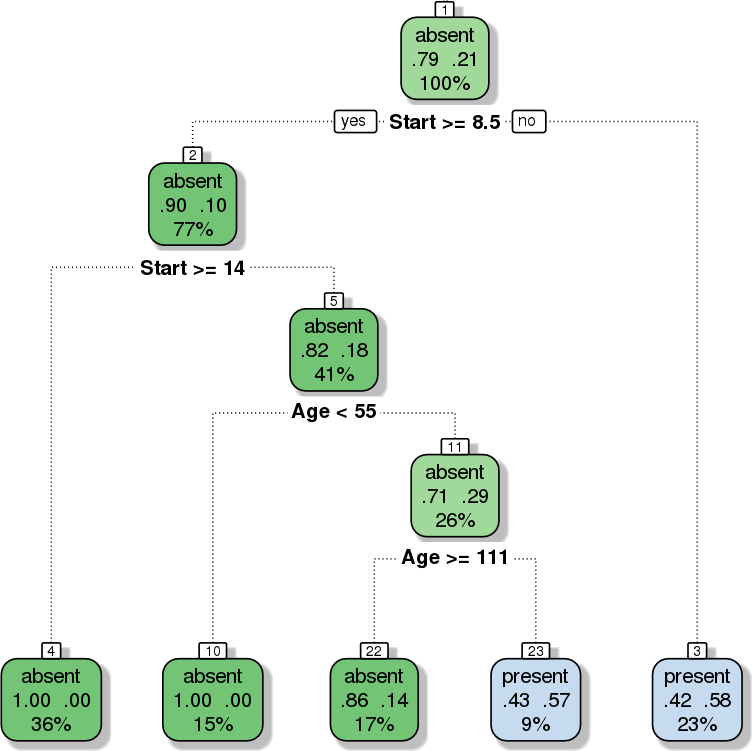
\includegraphics[width=0.85\textwidth]{images/DV/class_kyphosis_tree2.png}
\caption[\small Decision Tree: classification scheme for the kyphosis dataset ]{\small Decision Tree: classification scheme for the kyphosis dataset (personal file).} \label{fig:ex_dt_kyp}
\end{figure}
\afterpage{\FloatBarrier}
\vfill
\begin{figure}[H]
\centering
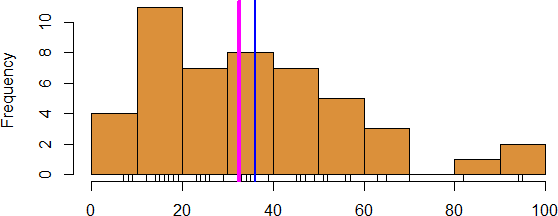
\includegraphics[width=0.85\textwidth]{images/DV/Histogram_of_GAS.png}
\caption[\small Histogram: artificial dataset ]{\small Histogram: artificial dataset (personal file).} \label{fig:ex_hist_GAS}
\end{figure}
\afterpage{\FloatBarrier}
\vfill 
\newpage
\vfill
\begin{figure}[H]
\centering
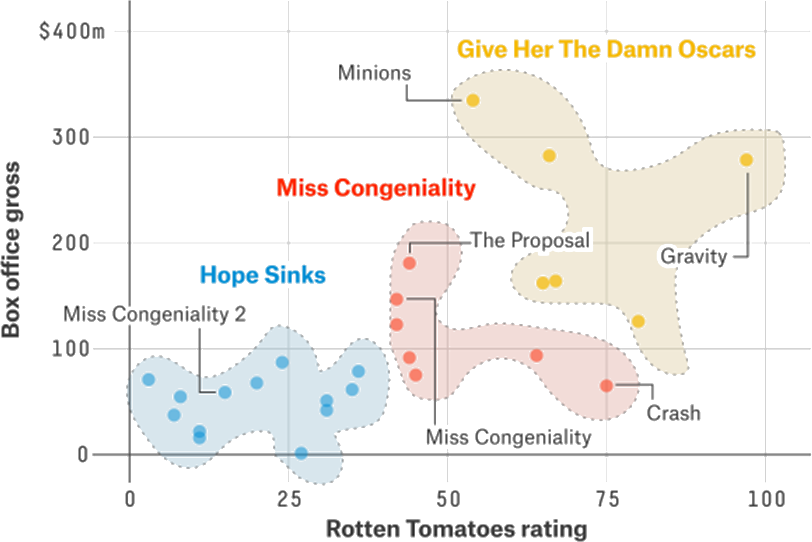
\includegraphics[width=0.7\textwidth]{images/DV/clustering.png}
\caption[\small Clustering Scatterplot: clustering of Sandra Bullock movies ]{\small Clustering Scatterplot: clustering of Sandra Bullock movies, by Rotten Tomatoes rating and inflation-adusted domestic gross (fivethirtyeight.com).} \label{fig:ex_cl_bul}
\end{figure}
\afterpage{\FloatBarrier}
\vfill
\begin{figure}[H]
\centering
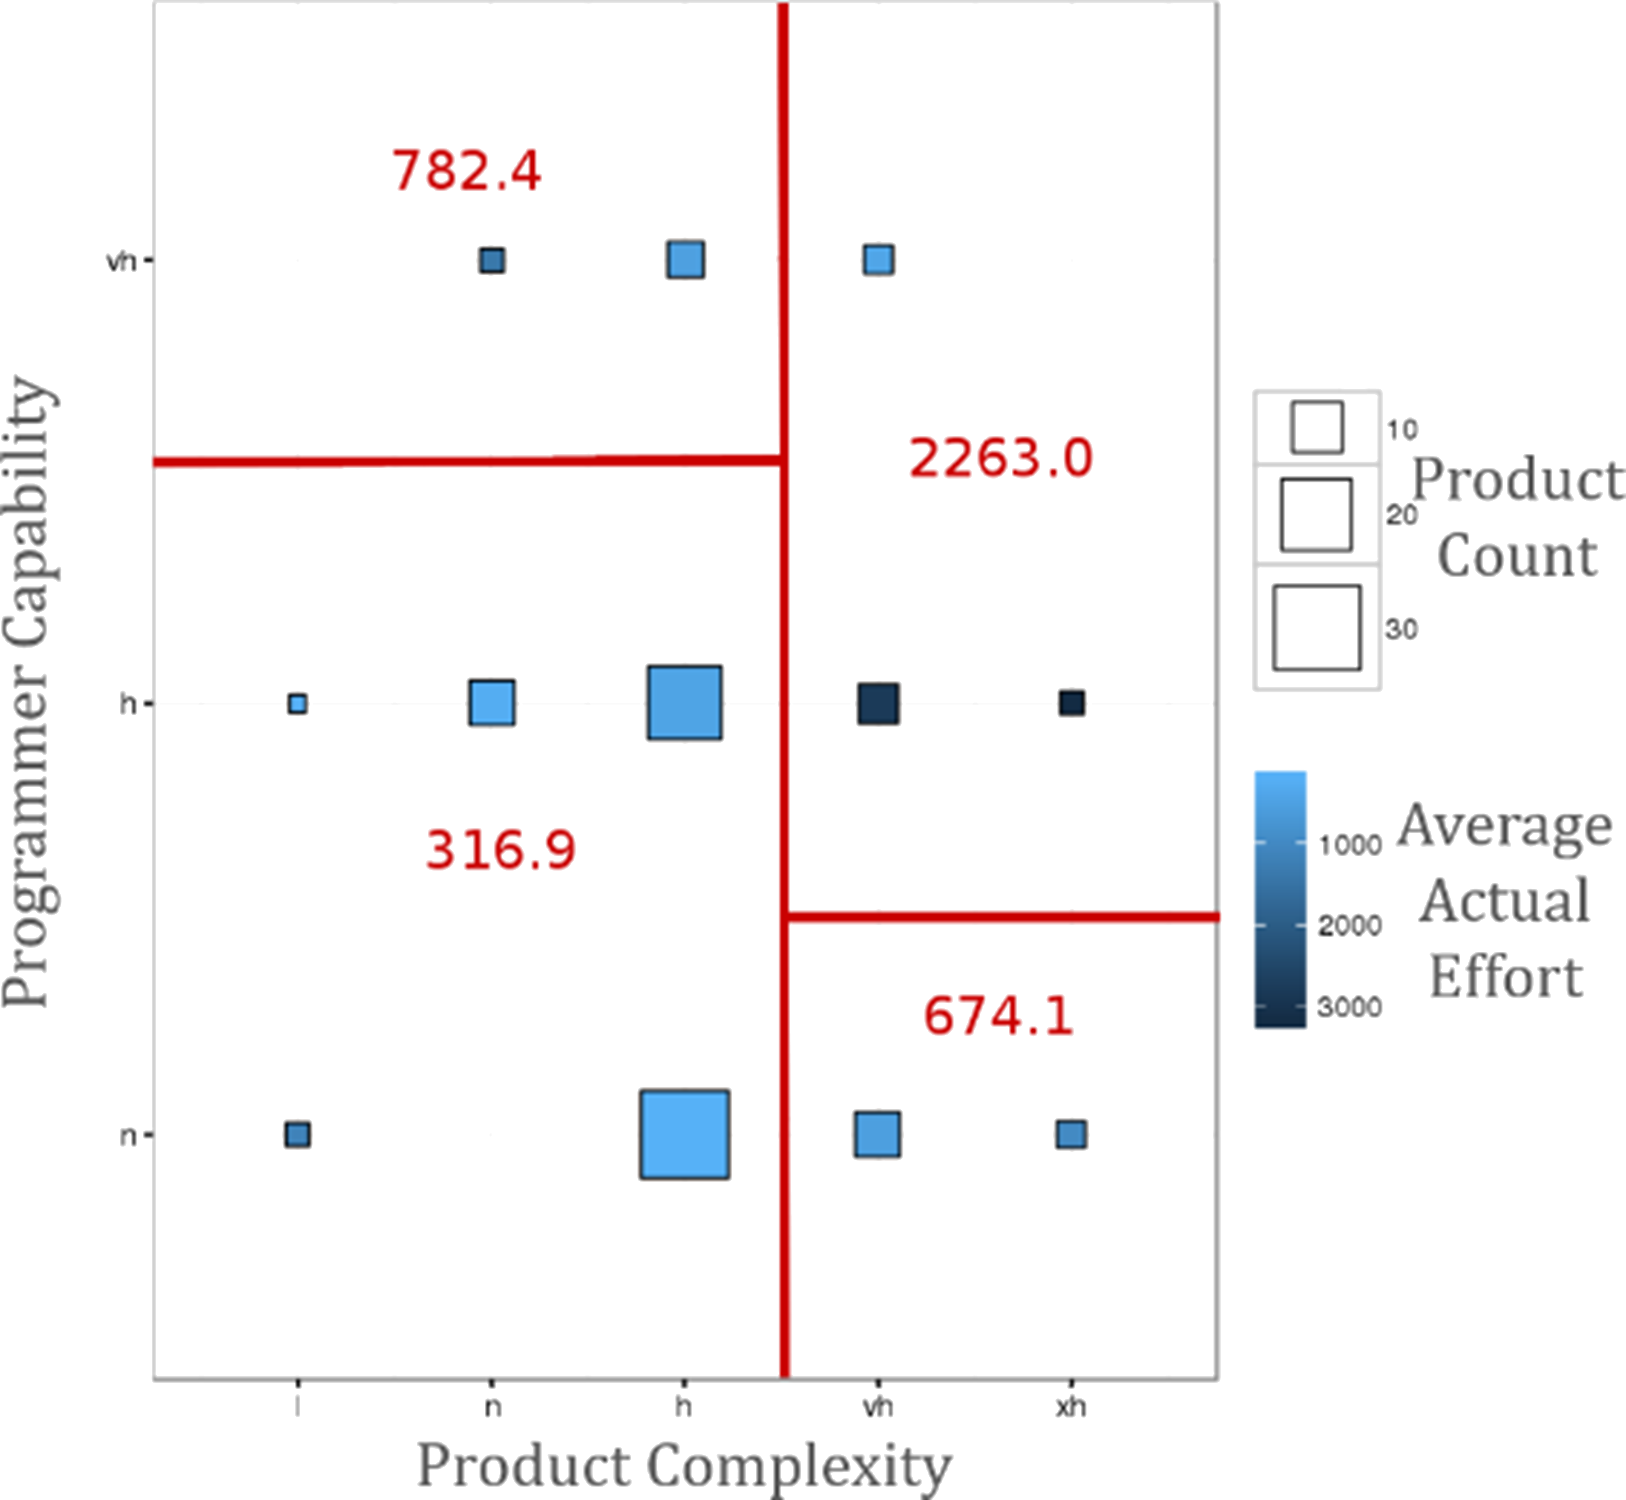
\includegraphics[width=0.7\textwidth]{images/DV/combined.png}
\caption[\small Decision Tree Bubble Chart: NASA's COCOMO dataset ]{\small Decision Tree Bubble Chart: estimated average project effort (in red) over-layed over product complexity, programmer capability, and product count in NASA's COCOMO dataset (personal file).} \label{fig:ex_sdt_comps}
\end{figure}
\afterpage{\FloatBarrier}
\vfill
\newpage
\vfill
\begin{figure}[H]
\centering
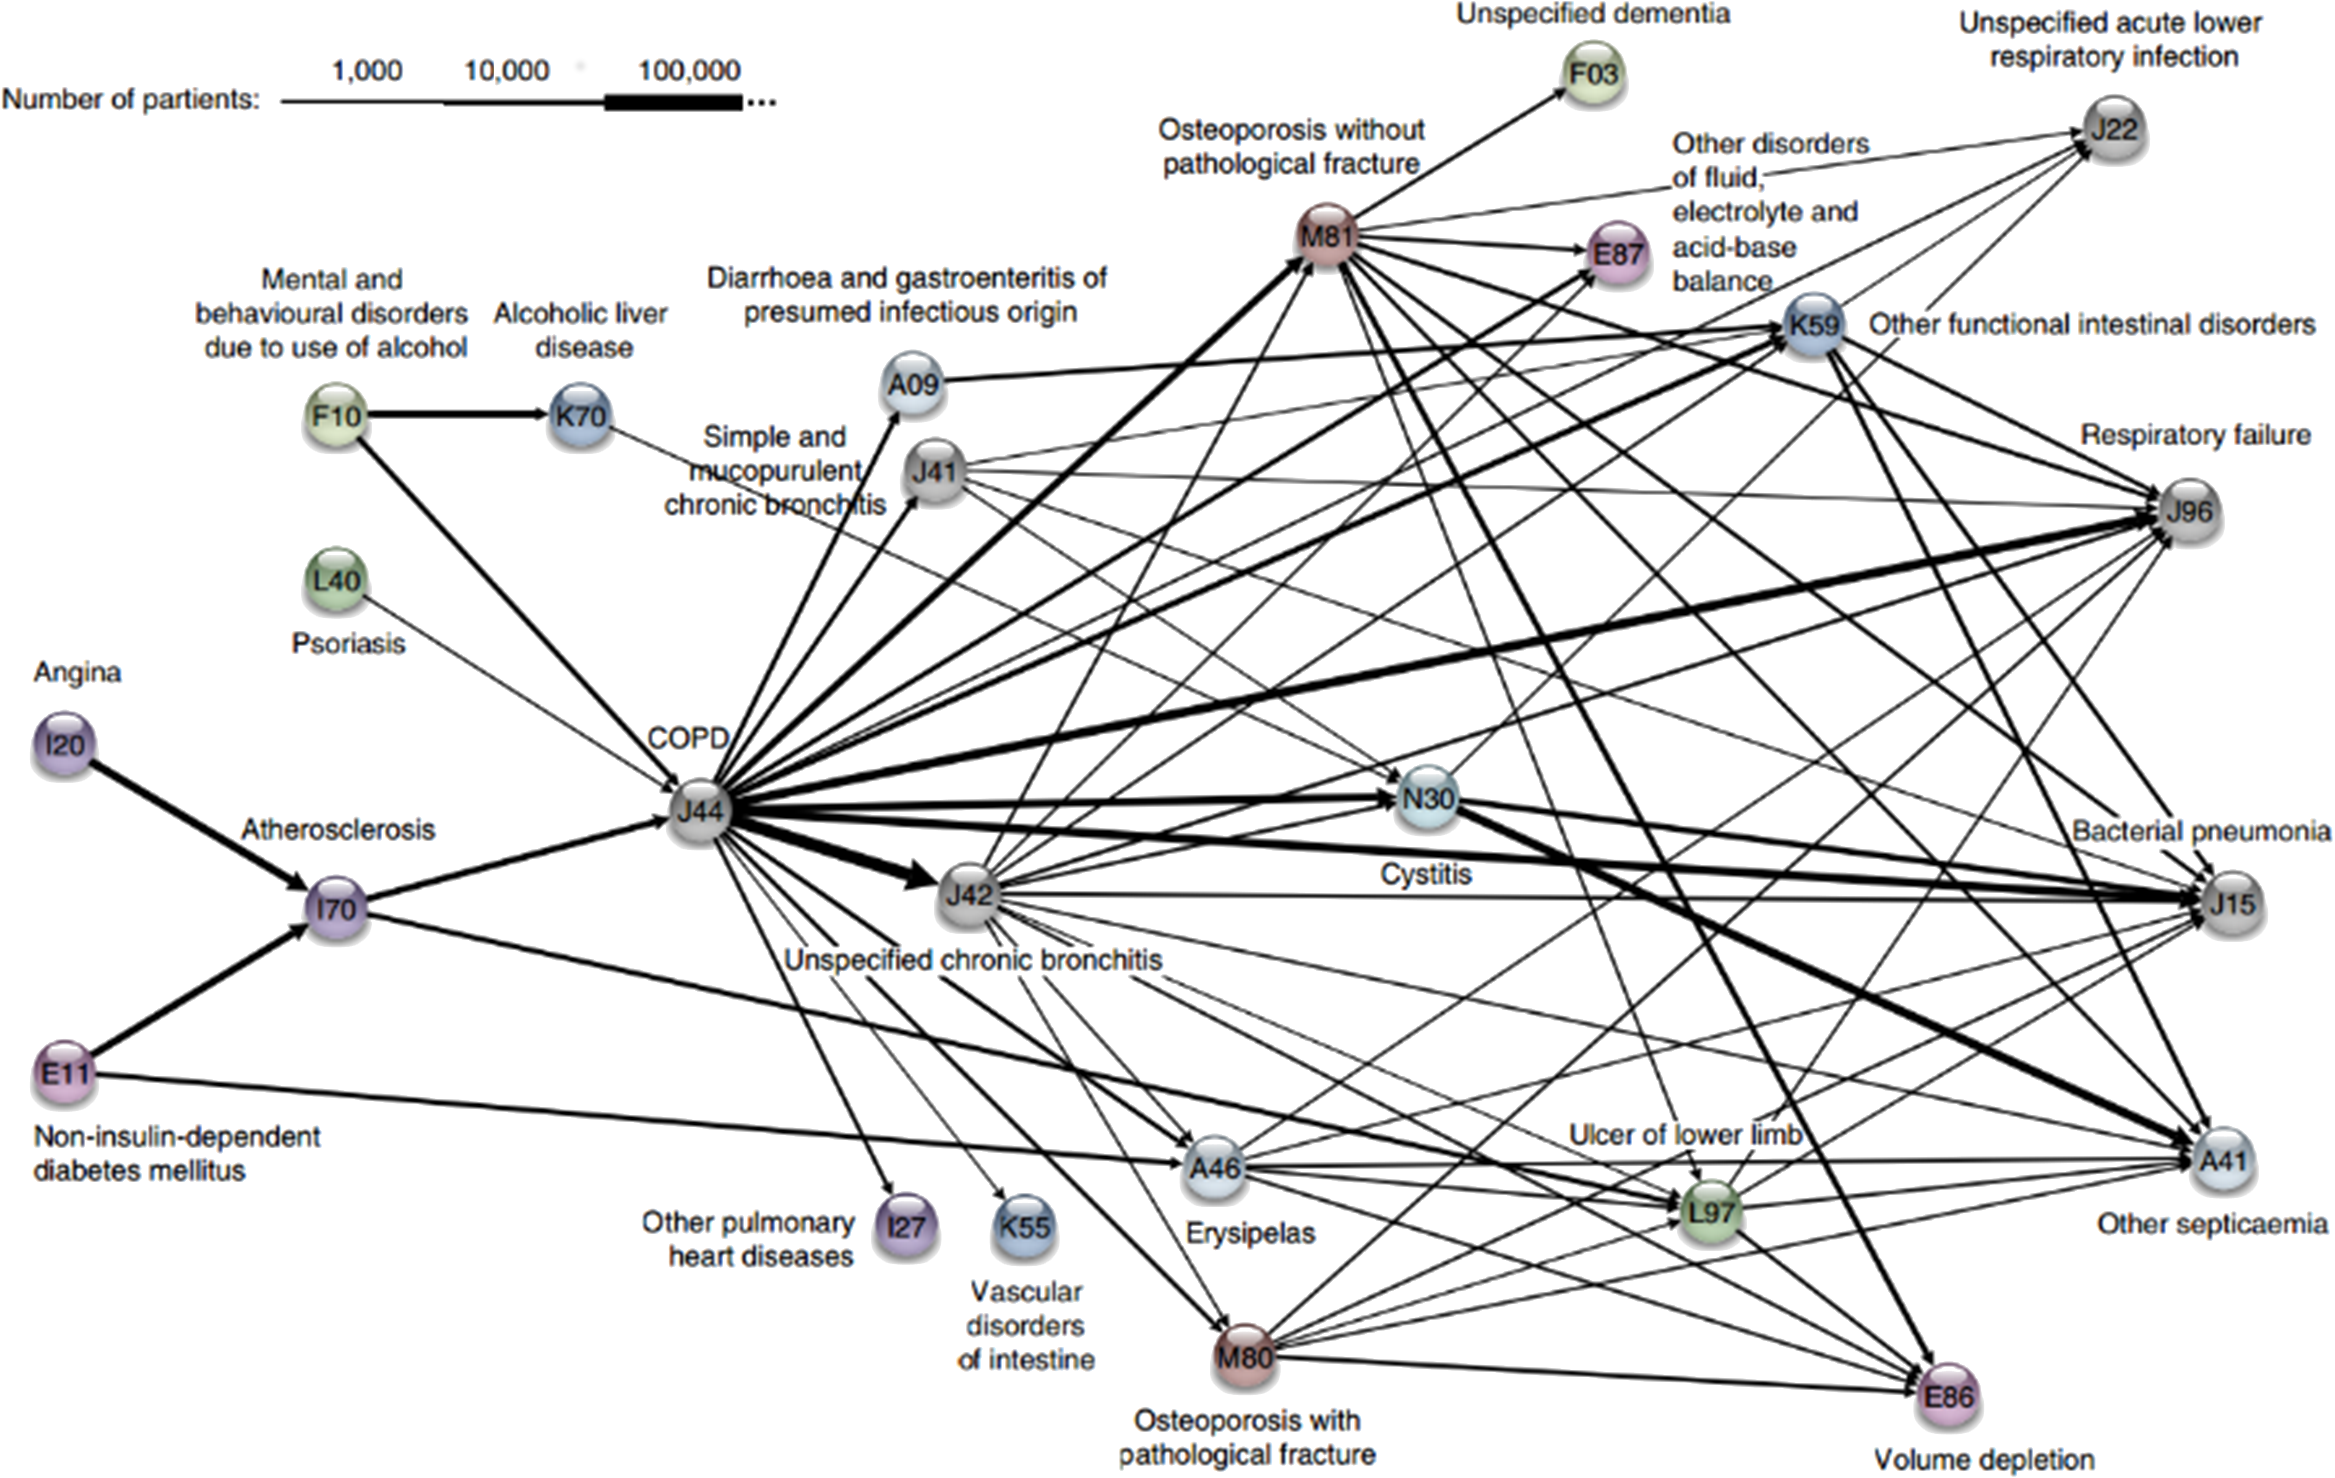
\includegraphics[width=0.95\textwidth]{images/DV/COPD.png}
\caption[\small Association Rule Network: Danish Medical Dataset ]{\small Association Rule Network: diagnosis network around COPD in the Danish Medical Dataset (A.B. Jensen \textit{et al}).} \label{fig:ex_arn_copd}
\end{figure}
\afterpage{\FloatBarrier}
\vfill
\begin{figure}[H]
\centering
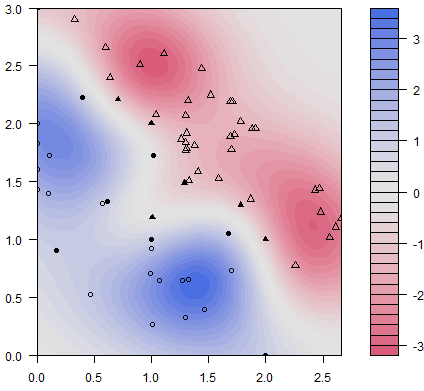
\includegraphics[width=0.6\textwidth]{images/DV/fig9.png}
\caption[\small Classification Scatterplot: artificial dataset ]{\small Classification Scatterplot: artificial dataset (personal file).} \label{fig:ex_cs_SVM}
\end{figure}
\afterpage{\FloatBarrier}
\vfill
\newpage
\vfill
\begin{figure}[H]
\centering
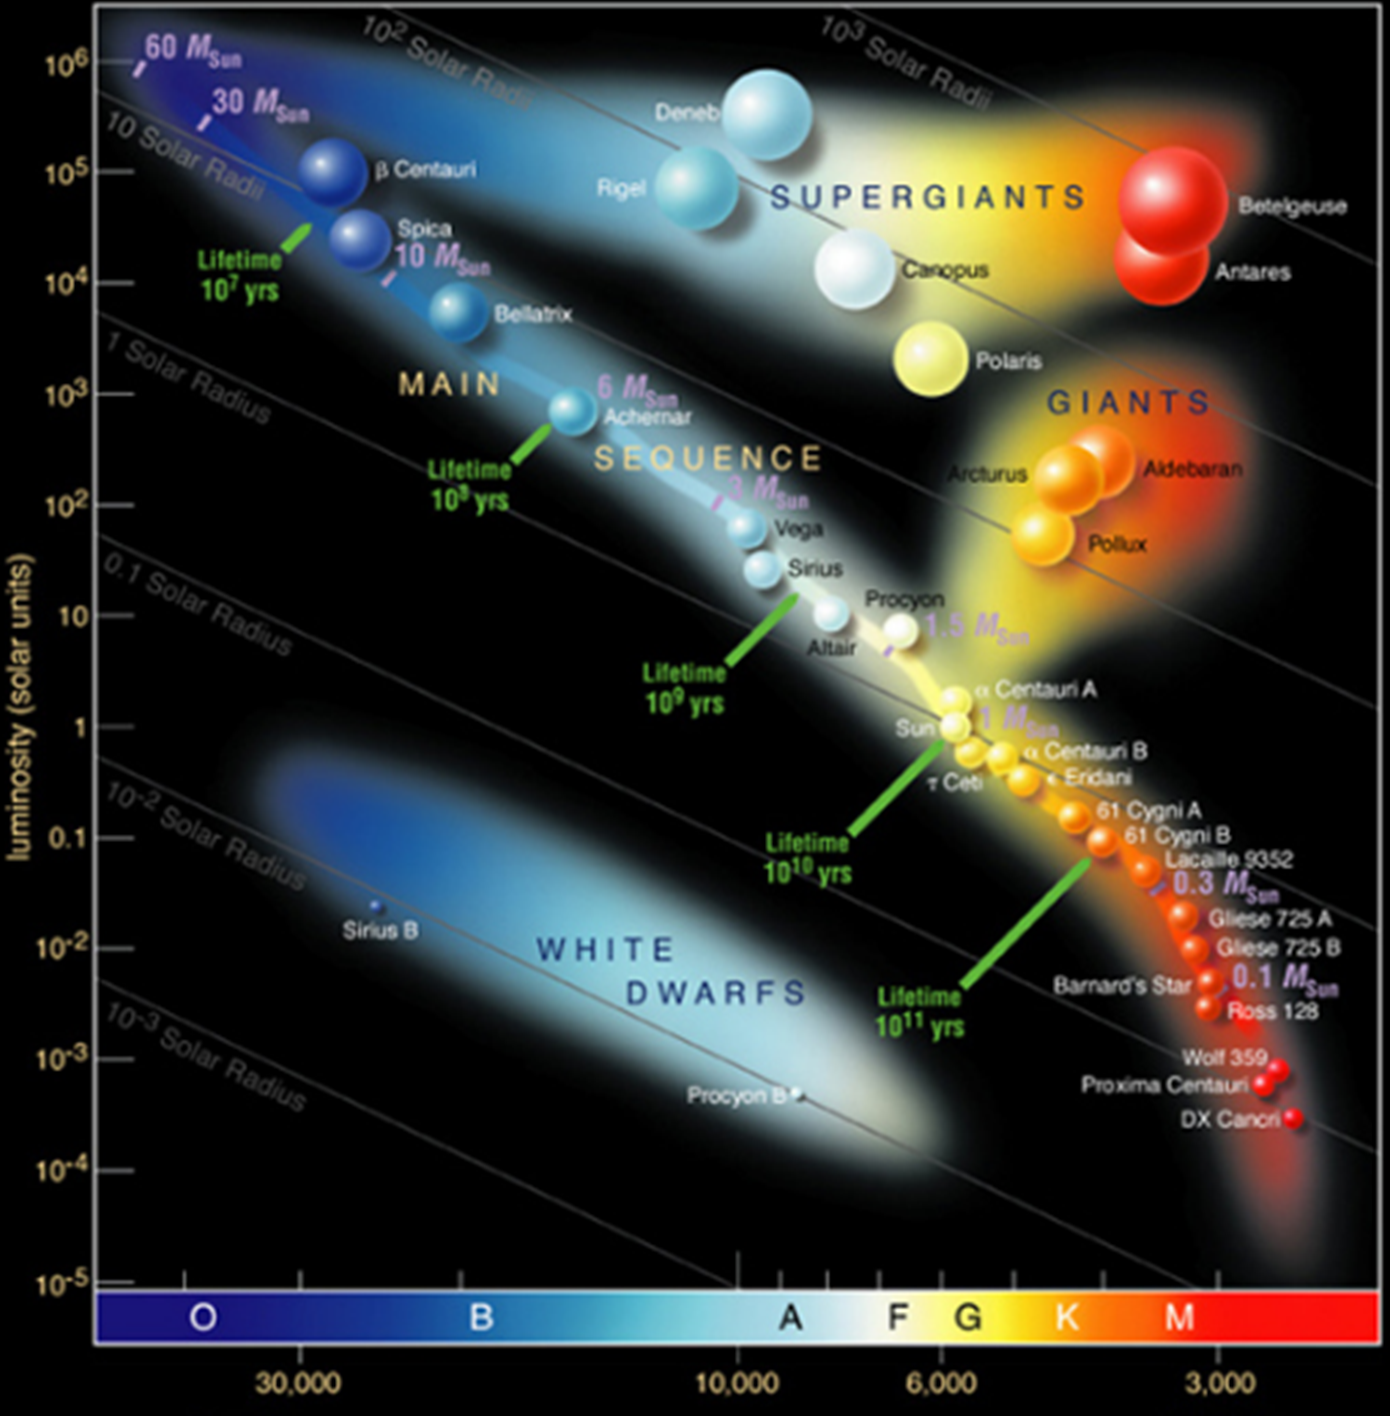
\includegraphics[width=0.65\textwidth]{images/DV/HR.png}
\caption[\small Classification Bubble Chart: Hertzsprung-Russell Diagram ]{\small Classification Bubble Chart: Hertzsprung-Russell Diagram (European Southern Observatory).} \label{fig:ex_bc_HR}
\end{figure}
\afterpage{\FloatBarrier}
\vfill
\begin{figure}[H]
\centering
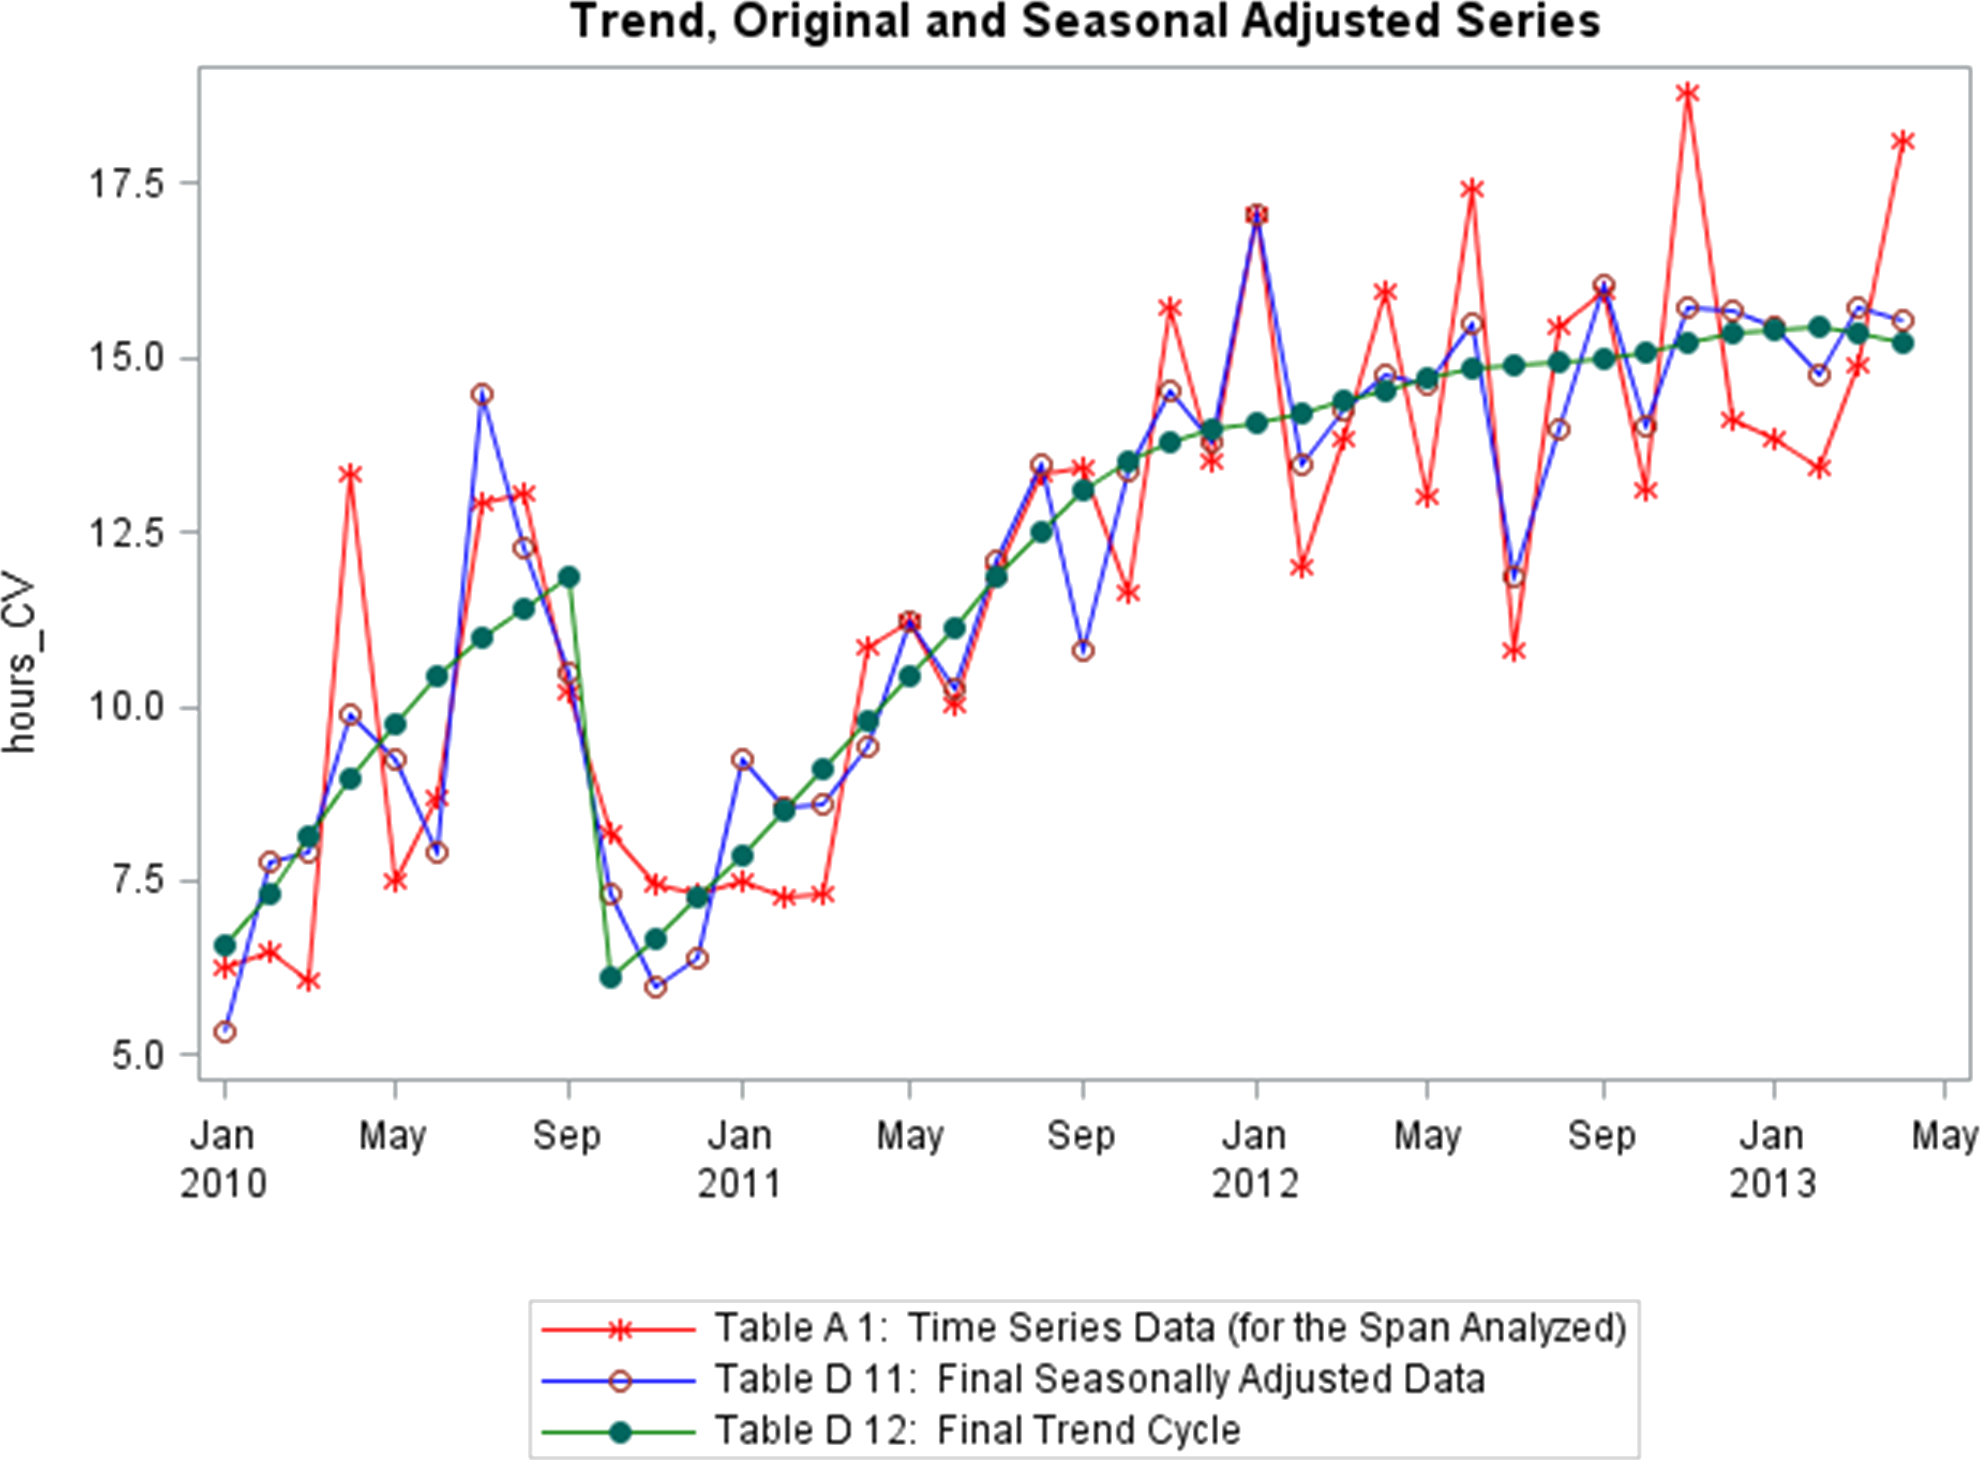
\includegraphics[width=0.65\textwidth]{images/DV/TS.png}
\caption[\small Time Series: trend, seasonality, and shifts ]{\small Time Series: trend, seasonality, and shifts (personal file).} \label{fig:ex_ts_cv}
\end{figure}
\afterpage{\FloatBarrier}
\vfill
\newpage


\subsubsection{Case Study: Reliability of Canadian Consular Network Data}
The \textit{Canadian Consular Network} provides services to Canadians travelling or living abroad (loss of a passport, need for urgent medical care, complications due to an arrest, or other emergencies). Consular officials can be reached 24 hours a day, seven days a week, at more than 260 points of service in 150 countries and through the \textit{Emergency Watch and Response Centre} in Ottawa. The type and amount of help that consular officials can provide depends on the situation and may be affected by natural disasters, political unrest, and the laws in effect in other countries.
\newl Within \textit{Global Affairs Canada} (GAC), the Consular Corporate Management and Innovation group (CCMI) uses COSMOS, a software application that tracks consular activity statistics. COSMOS is used to enable consulates to provide assistance to their consular clients and to help identify where the workload stresses are located. It can also be used to provide basic statistics for requests from journalists and others.
\newl COMIP (a COSMOS module) tracks the time required by employees to perform consular tasks. This data, in one form or another, stretches back over approximately twenty years (from 2016). It is currently used to 
determine the effectiveness of mission consular programs, to identify weaknesses to be resolved through HR, training and other solutions, and to evaluate resources need in missions -- COMIP is the pivotal element when determining whether to staff, delete, or create positions. The software is scheduled to be updated/replaced (late 2016), and GAC would like to use this opportunity to determine if the current system meets their needs, and if not, how it could be improved. \newl 
The data of primary interest for consular management is contained in 4 COMIP tables: the logs of mission activities (\textbf{cases}, \textbf{services}, and \textbf{programs}), as well as the daily and monthly time spent on these mission activities, by employee. In these tables, data is available across a time span of 10 years, from 2005--2014; however, a 2010 system upgrade changed the categories relating to cases and services, resulting in a break in the dataset at this time. \newl 
In data analytical endeavours, the quality of the output is affected by the quality of the input, especially when it is self-reported (such as is the case with COMIP). CCMI understands that monthly log data has, in some sense, more inherent validity than daily log data as it must be reviewed by management before being submitted into the system -- this oversight may be sufficient to ensure greater validity of that data. 
Daily log data by contrast may be entered less diligently as they are not required to produce a monthly log. \newl Abandoning daily log data altogether is not a solution as it is impossible to create monthly log data that accurately reflects the reality of monthly work in the mission without using (some) information from employees about their daily work during the month. Daily data, thus, is used \textit{de facto} to create the monthly logs. \newl As a result, while certain types of consular data analysis may be conducted using monthly aggregates, data validation has to occur at the daily data level. In this case study, we present various data visualisations that were produced to study the reliability and validity of COMIP data. \newpage\noindent
\paragraph{Contents}
\begin{quote}
Basic Check - Data Gaps \\
Entire Dataset Review \\
Mission-Level Dataset Review  \\
Plausibility of Work Hours \\
Employee-Level Dataset Review 
\end{quote}

\phantomsection
\begin{thebibliography}{99}
\bibitem{DV_M2} Malamed, C., \newhref{http://understandinggraphics.com}{Understanding Graphics}.
\bibitem{DV_KW} Krygier, J., Wood, D., [2016], Making Maps: A Visual Guide to Map Design for GIS, Guilford Press.
\bibitem{DV_IDV} \newhref{https://en.wikipedia.org/wiki/Interactive_data_visualization}{Interactive Data Visualization} on Wikipedia.
\bibitem{DV_S} Simmon, R. [2013], \newhref{https://earthobservatory.nasa.gov/blogs/elegantfigures/2013/03/14/is-animation-an-effective-tool-for-data-visualization/}{Is animation an effective tool for data visualization?}, NASA's Earth Observatory. 
\bibitem{DV_H} Healey, C.G., \newhref{https://www.csc2.ncsu.edu/faculty/healey/PP/}{Perception in Visualization}
\bibitem{DV_P} \newhref{http://dataphys.org/list/}{Data Physicalizations}
\bibitem{DV_T1} Tufte, E. [2001], The Visual Display of Quantitative Information, Graphics Press.
\bibitem{DV_H2} Hu, D. [1954], How to Lie With Statistics, Norton.
\bibitem{DV_T2} Tufte, E. [2008], Beautiful Evidence, Graphics Press.
\bibitem{DV_NK} Nussbaumer Knaflic, C. [2015], Storytelling with Data, Wiley.
\bibitem{DV_C1} Cairo, A. [2013], The Functional Art, New Riders.
\bibitem{DV_C2} Cairo, A. [2016], The Truthful Art, New Riders.
\bibitem{DV_M} Meireilles, I. [2013], Design for Information, Rockport.
\bibitem{DV_50} \newhref{http://www.webdesignerdepot.com}{50 Great Examples of Data Visualization}. 
\bibitem{DV_K} Kirk, A., \newhref{http://www.visualisingdata.com}{Visualising Data}.
\bibitem{DV_Y} Yau, N., \newhref{http://flowingdata.com}{FlowingData}. 
\bibitem{DV_DV} \newhref{https://en.wikipedia.org/wiki/Data_visualization}{Data Visualization} on Wikipedia.
\bibitem{DV_MG} \newhref{https://en.wikipedia.org/wiki/Misleading_graphs}{Misleading Graphs} on Wikipedia.
\bibitem{DV_P2} Prabhakaran, S., \newhref{http://r-statistics.co/Top50-Ggplot2-Visualizations-MasterList-R-Code.html}{Top 50 ggplot2 Visualizations}. 
\bibitem{DV_M3} Miller, M. [2017], The problem with Interactive graphics, Co.Design
\bibitem{DV_W} Wickham, H. [2016], ggplot2: Elegant Graphics for Data Analysis (2nd ed), Springer.
\bibitem{DV_G} Gorelik, B., Data Visualization (blog).
\bibitem{DV_AIM} Miller, A.I. [2012], \newhref{https://www.theguardian.com/science/blog/2012/jul/17/henri-poincare-einstein-picasso?newsfeed=true}{Henri Poincar\'e: the unlikely link between Einstein and Picasso}, in The Guardian. 
\bibitem{DV_WSC} Wexler, S., Shaffer, J., Cotgreave, A. [2017], the Big Book of Dashboards, Wiley. 
\end{thebibliography}
\setboolean{@twoside}{false}
\includepdf[pages={1-8},offset={50 -40}]{documents/GAC_captions.pdf}
\setboolean{@twoside}{true}



